\documentclass[tikz, border=15pt]{standalone}
\usepackage{xcolor}
\usetikzlibrary{arrows.meta}

% Define color palette
\definecolor{bgcolor}{RGB}{15, 23, 42}       % Deep Slate Blue
\definecolor{laserred}{RGB}{255, 48, 48}    % High-intensity Laser Red
\definecolor{glasscyan}{RGB}{165, 243, 252} % Glass Splitter / Compensator
\definecolor{mirrorblue}{RGB}{186, 230, 253}% Reflective coating
\definecolor{metalbg}{RGB}{71, 85, 105}     % Dark Steel
\definecolor{metalfg}{RGB}{148, 163, 184}   % Light Steel

\begin{document}
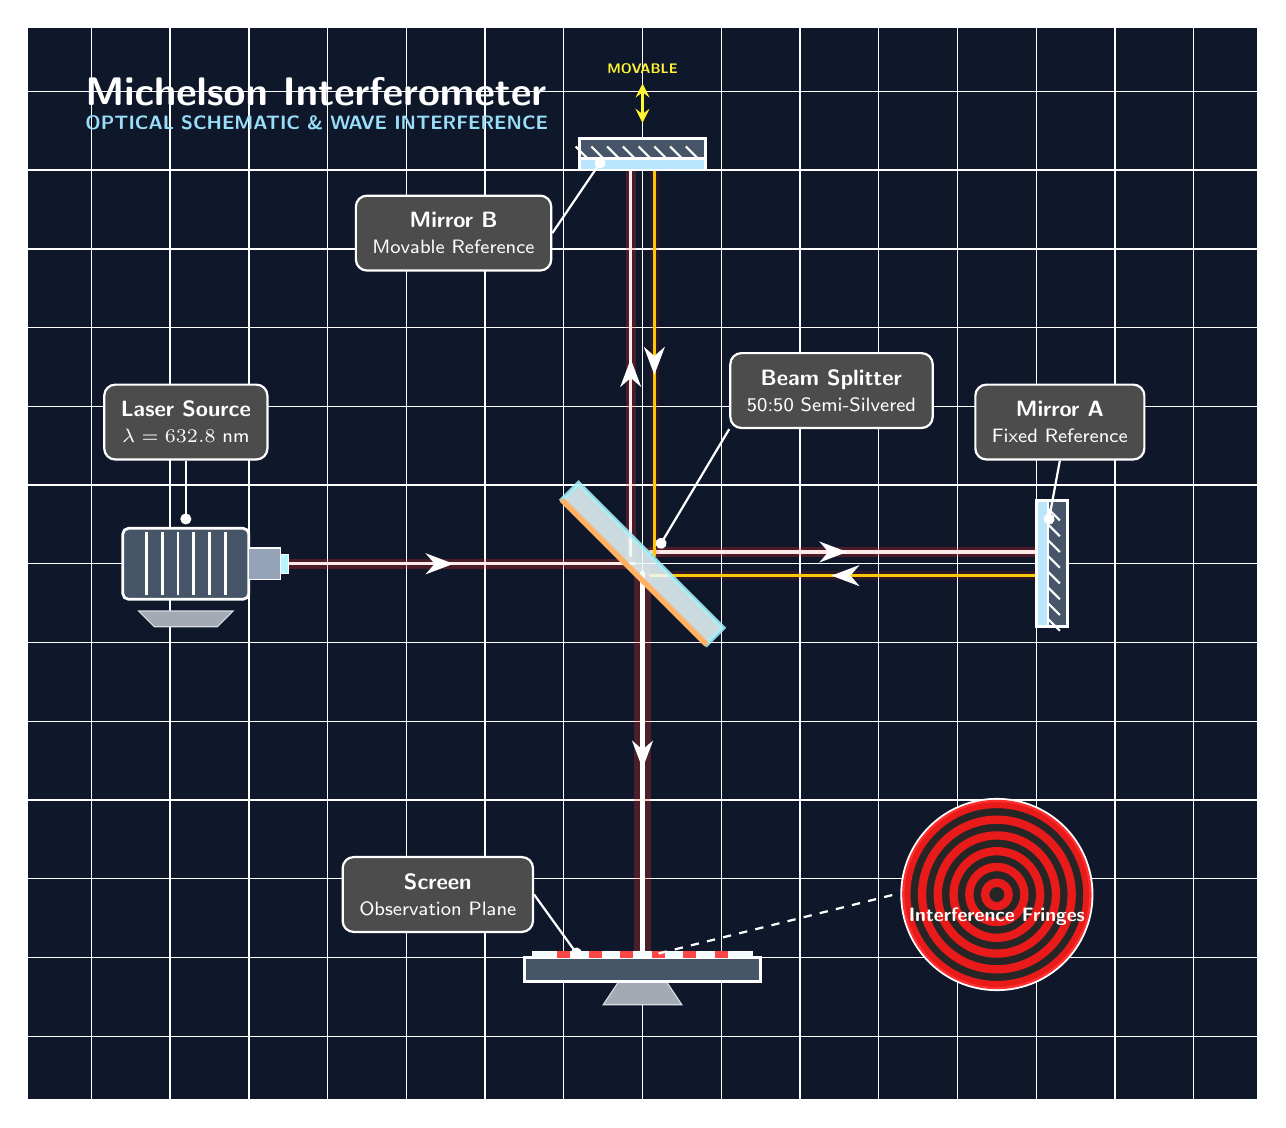
\begin{tikzpicture}

% Styles
\tikzset{
    beam-glow/.style={
        line width=3.5pt,
        laserred,
        opacity=0.25,
        line cap=round
    },
    beam-core/.style={
        line width=1.2pt,
        white!90!laserred,
        line cap=round
    },
    arrow-style/.style={
        -{Stealth[scale=1.2]},
        white,
        line width=1.2pt
    },
    hud-card/.style={
        fill=black!70,
        draw=white!25,
        rounded corners=4pt,
        line width=0.8pt,
        inner sep=6pt,
        text=white,
        font=\sffamily\footnotesize
    },
    leader-line/.style={
        white!50,
        line width=0.8pt,
        -{Circle[scale=0.8]}
    }
}

% 1. Background and Grid
\fill[bgcolor] (-7.8, -6.8) rectangle (7.8, 6.8);
\draw[white!4, step=1.0, line width=0.5pt] (-7.8, -6.8) grid (7.8, 6.8);

% 2. Title Block
\node[anchor=west, text=white, font=\sffamily\Large\bfseries] at (-7.2, 6.0) {Michelson Interferometer};
\node[anchor=west, text=cyan!40, font=\sffamily\scriptsize\bfseries] at (-7.2, 5.6) {OPTICAL SCHEMATIC \& WAVE INTERFERENCE};

% 3. Light Beams (Glow and Core) - Draw first so they sit behind components
% Laser to Beam Splitter
\draw[beam-glow] (-4.6, 0) -- (-0.1, 0);
\draw[beam-core] (-4.6, 0) -- (-0.1, 0);

% Arm A (Reference Arm) - Go
\draw[beam-glow] (0.1, 0.15) -- (5.0, 0.15);
\draw[beam-core] (0.1, 0.15) -- (5.0, 0.15);

% Arm A (Reference Arm) - Return
\draw[beam-glow, opacity=0.15, laserred!80!black] (5.0, -0.15) -- (0.1, -0.15);
\draw[beam-core, yellow!80!red] (5.0, -0.15) -- (0.1, -0.15);

% Arm B (Movable Arm) - Go
\draw[beam-glow] (-0.15, 0.1) -- (-0.15, 5.0);
\draw[beam-core] (-0.15, 0.1) -- (-0.15, 5.0);

% Arm B (Movable Arm) - Return
\draw[beam-glow, opacity=0.15, laserred!80!black] (0.15, 5.0) -- (0.15, 0.1);
\draw[beam-core, yellow!80!red] (0.15, 5.0) -- (0.15, 0.1);

% Combined Beam to Screen
\draw[beam-glow, line width=6pt, laserred!90!orange] (0, -0.12) -- (0, -5.0);
\draw[beam-core, line width=2pt, white] (0, -0.12) -- (0, -5.0);

% 4. Directional Arrows
\draw[arrow-style] (-2.6, 0) -- (-2.4, 0);
\draw[arrow-style] (2.4, 0.15) -- (2.6, 0.15);
\draw[arrow-style] (2.6, -0.15) -- (2.4, -0.15);
\draw[arrow-style] (-0.15, 2.4) -- (-0.15, 2.6);
\draw[arrow-style] (0.15, 2.6) -- (0.15, 2.4);
\draw[arrow-style] (0, -2.4) -- (0, -2.6);

% 5. Physical Components

% Laser Source
\begin{scope}[shift={(-5.8, 0)}]
    % Mount/Base
    \draw[fill=metalbg!50, draw=metalbg!20] (-0.6, -0.6) -- (-0.4, -0.8) -- (0.4, -0.8) -- (0.6, -0.6) -- cycle;
    % Main Body
    \draw[fill=metalbg, draw=white!20, rounded corners=2pt, line width=1pt] (-0.8, -0.45) rectangle (0.8, 0.45);
    % Heat sink fins
    \foreach \x in {-0.5, -0.3, -0.1, 0.1, 0.3, 0.5} {
        \draw[white!20, line width=1pt] (\x, -0.4) -- (\x, 0.4);
    }
    % Output Nozzle
    \draw[fill=metalfg, draw=white!30] (0.8, -0.2) rectangle (1.2, 0.2);
    \draw[fill=glasscyan!80, draw=white] (1.2, -0.12) rectangle (1.3, 0.12);
\end{scope}

% Beam Splitter
\begin{scope}[rotate=45]
    % Glass plate
    \draw[fill=glasscyan!20, draw=glasscyan, opacity=0.85, line width=1.5pt] (-0.15, -1.3) rectangle (0.15, 1.3);
    % Semi-reflective coating (labeled side)
    \draw[line width=2pt, draw=orange!60!white] (-0.15, -1.3) -- (-0.15, 1.3);
\end{scope}

% Mirror A (Fixed Reference Mirror)
\begin{scope}[shift={(5.0, 0)}]
    % Backing
    \draw[fill=metalbg, draw=white!20, line width=1pt] (0.15, -0.8) rectangle (0.4, 0.8);
    % Reflective Surface
    \draw[fill=mirrorblue, draw=white, line width=1pt] (0, -0.8) rectangle (0.15, 0.8);
    % Back shading
    \foreach \y in {-0.7,-0.5,-0.3,-0.1,0.1,0.3,0.5,0.7} {
        \draw[white!20, line width=0.8pt] (0.15, \y) -- (0.3, \y-0.15);
    }
\end{scope}

% Mirror B (Movable Mirror)
\begin{scope}[shift={(0, 5.0)}]
    % Backing
    \draw[fill=metalbg, draw=white!20, line width=1pt] (-0.8, 0.15) rectangle (0.8, 0.4);
    % Reflective Surface
    \draw[fill=mirrorblue, draw=white, line width=1pt] (-0.8, 0) rectangle (0.8, 0.15);
    % Back shading
    \foreach \x in {-0.7,-0.5,-0.3,-0.1,0.1,0.3,0.5,0.7} {
        \draw[white!20, line width=0.8pt] (\x, 0.15) -- (\x-0.15, 0.3);
    }
    % Motion Indicator Arrow
    \draw[<->, >=stealth, draw=yellow!80!white, line width=1.2pt] (0, 0.6) -- (0, 1.1);
    \node[text=yellow!80!white, font=\sffamily\tiny\bfseries, above] at (0, 1.1) {MOVABLE};
\end{scope}

% Screen (Detector)
\begin{scope}[shift={(0, -5.0)}]
    % Mount
    \draw[fill=metalbg!50, draw=metalbg!20] (-0.3, -0.3) -- (-0.5, -0.6) -- (0.5, -0.6) -- (0.3, -0.3) -- cycle;
    % Plate
    \draw[fill=metalbg, draw=white!20, line width=1pt] (-1.5, -0.3) rectangle (1.5, 0);
    % White projection surface
    \draw[fill=white!95!cyan, draw=white] (-1.4, 0) rectangle (1.4, 0.08);
    % Projected Fringes
    \foreach \x in {-1.0, -0.6, -0.2, 0.2, 0.6, 1.0} {
        \fill[red!90!white, opacity=0.8] (\x-0.08, 0) rectangle (\x+0.08, 0.08);
    }
\end{scope}

% 6. Interference Pattern Zoom-in (Quadrant IV)
\begin{scope}[shift={(4.5, -4.2)}]
    % Dotted connection to screen
    \draw[white!30, dashed, line width=0.8pt] (-4.5, -0.8) -- (-1.3, 0);
    
    % Border
    \draw[fill=black!85, draw=white!40, line width=1.5pt] (0,0) circle (1.2);
    
    % Fringes
    \foreach \r in {0.15, 0.35, 0.55, 0.75, 0.95, 1.15} {
        \draw[red!90!white, line width=3pt, opacity=0.9] (0,0) circle (\r);
    }
    
    % Label
    \node[white, font=\sffamily\scriptsize\bfseries, below=1.4] at (0,0) {Interference Fringes};
\end{scope}

% 7. Labels & Glassmorphic HUD Cards
% Laser
\node[hud-card, align=center] (L-Label) at (-5.8, 1.8) {\textbf{Laser Source}\\\scriptsize $\lambda = 632.8$ nm};
\draw[leader-line] (L-Label.south) -- (-5.8, 0.5);

% Beam Splitter
\node[hud-card, align=center] (BS-Label) at (2.4, 2.2) {\textbf{Beam Splitter}\\\scriptsize 50:50 Semi-Silvered};
\draw[leader-line] (BS-Label.south west) -- (0.2, 0.2);

% Mirror A
\node[hud-card, align=center] (MA-Label) at (5.3, 1.8) {\textbf{Mirror A}\\\scriptsize Fixed Reference};
\draw[leader-line] (MA-Label.south) -- (5.15, 0.5);

% Mirror B
\node[hud-card, align=center] (MB-Label) at (-2.4, 4.2) {\textbf{Mirror B}\\\scriptsize Movable Reference};
\draw[leader-line] (MB-Label.east) -- (-0.5, 5.15);

% Screen
\node[hud-card, align=center] (S-Label) at (-2.6, -4.2) {\textbf{Screen}\\\scriptsize Observation Plane};
\draw[leader-line] (S-Label.east) -- (-0.8, -5.0);

\end{tikzpicture}
\end{document}
